%usage: pdflatex <datei>.tex

\documentclass[11pt,a4paper]{scrartcl}
\usepackage{graphicx,color,rotating}
\usepackage{graphics}
\usepackage{wrapfig}
\usepackage[utf8]{inputenc}
\usepackage{amsfonts}
\usepackage{amsmath}
\usepackage{dsfont}
\usepackage{url}
\usepackage{listings}
\usepackage{hyperref}
\hyphenation{}

\definecolor{darkblue}{rgb}{0,0,.6}
\definecolor{darkred}{rgb}{.6,0,0}
\definecolor{darkgreen}{rgb}{0,.6,0}
\definecolor{red}{rgb}{.98,0,0}

\lstloadlanguages{C}

\makeatletter% --> De-TeX-FAQ
\renewcommand*{\lstlistoflistings}{%
  \begingroup
    \if@twocolumn
      \@restonecoltrue\onecolumn
    \else
      \@restonecolfalse
    \fi
    \lol@heading
    \setlength{\parskip}{\z@}%
    \setlength{\parindent}{\z@}%
    \setlength{\parfillskip}{\z@ \@plus 1fil}%
    \@starttoc{lol}%
    \if@restonecol\twocolumn\fi
  \endgroup
}
\makeatother% --> \makeatletter

\lstnewenvironment{code}[1][]
{\smallskip\lstset{
	caption = #1,
	language=C,
	basicstyle=\footnotesize\ttfamily,
  	commentstyle=\itshape\color{darkgreen},
  	keywordstyle=\bfseries\color{darkblue},
  	stringstyle=\color{darkred},
  	tabsize=4,
  	showspaces=false,
  	showtabs=false,
  	columns=fixed,
  	frame=none,
	numbers=left,
  	numberstyle=\tiny,
  	breaklines=true,
  	showstringspaces=false,
  	xleftmargin=0cm}
	}
{\smallskip}

\setcounter{tocdepth}{3}

\begin{document}
\begin{titlepage}

\includegraphics[viewport = 90 575 0 0, scale = 1.2]{inanutshell.png}
\end{titlepage}
%\title{POTATOES\\system/development documentation}
%\author{Daniel Bader\\Vincenz Doelle\\Johannes Schamburger\\Dmitriy Traytel}
%\maketitle
%\pagebreak

\tableofcontents
\pagebreak

\section{Introduction}

\subsection{Motivation}
\textit{POTATOES}, a "Practical Oriented TeAching Tool" and "Operating (and) Educating System", aims to be a small but full fledged operating system based on the KISS \footnote{"Keep It Short and Simple"} principle. POTATOES's goal is not to replace established and advanced operating systems. It's purpose is to provide an easy to understand and well documented way to the design and implementation of operating systems.\\

Moreover, \textit{POTATOES}'s open source offers everyone the chance to use \textit{POTATOES} as a basis for own experiments or feature implementations. Thus, one can gain valuable practical experiences without disproportional high efforts and unforeseeable problems. Especially students for instance are welcome to implement some basic concepts of operating systems in order to get a deeper understanding of their theoretical knowledge.\\

Finally, the \textit{POTATOES} development team looks forward to working together with ambitious programmers and creative thinkers!

\pagebreak

\subsection{System}
\textit{POTATOES} is separated into four main kernel subsystems: 
\begin{enumerate}
	\item Process Management
	\item Memory Management
	\item Input/Output Interface
	\item File System
\end{enumerate}

Using a clear specification of the subsystems' interfaces and well defined communication directions, each subsystem can be maintained separately and independently from the remaining kernel components.\\

A schematic overview of the \textit{POTATOES}'s kernel and user space looks as follows:\\\\

\begin{figure}[h]
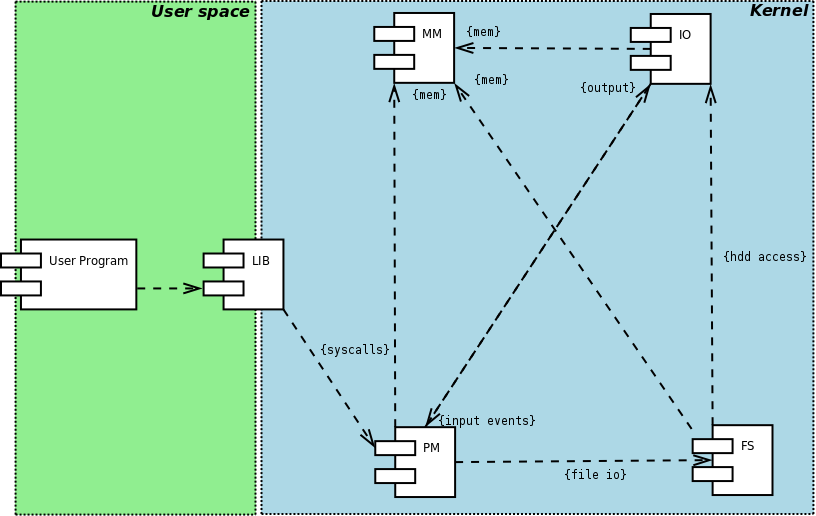
\includegraphics[width=\textwidth]{subsystems.png}
\caption{\textit{POTATOES}'s system overview}
\end{figure}
\pagebreak

\section{Memory Management}
An important task of the operating system is to manage the main memory.
Therefore it needs a memory manager which provides possibilities to programs and the kernel to allocate and free space dynamically.
\subsection{GDT}
The Global Descriptor Table (GDT) is an array of GDT entries describing the segmentation system.
Our boot loader \textit{GRUB} already creates a GDT for our system, but we need to create our own one because we don't know where \textit{GRUB} stores its GDT. Thus it could be accidentally overwritten.\\

\begin{code}[kernel/mm/mm.h]
struct gdt_entry {
	uint16 limit_low;
	uint16 base_low;
	uint8  base_middle;
	uint8  access;
	uint8  granularity;
	uint8  base_high;
} __attribute__((packed));
\end{code}
One GDT entry represents one certain segment (code or data) its start, end and the access levels.
So it is possible to divide the main memory into one segment for data and another segment for code, but as we don't actually use segmentation in \textit{POTATOES}, each segment has access to the whole address space (0x0 - 0xFFFFFFFF considering a 32bit processor). So we set the GDT entries to cover the whole address space.

\subsection{Paging}
Paging is used for two main goals: memory protection and virtual memory.

Virtual memory in general means that the address a program (or the kernel) gets by allocating some space is just a virtual address which is mapped on a physical one. For example an allocation call can return the address 0x00C00000 which is mapped on the physical address 0x00001200. So, each program can have an address space which starts at 0x00000000. The translation from virtual to physical address is done by the memory management unit (MMU)\footnote{\url{http://en.wikipedia.org/wiki/Memory_management_unit}}.
\subsubsection{Organization of frames}
In systems that use paging, the whole main memory is divided into fixed sized frames (in \textit{POTATOES} one frame has 4 KB).
To organize these frames, \textit{POTATOES} uses a bitmap structure. With that bitmap it is quite simple to mark frames as occupied/free or to find the first free frame.
\subsubsection{Organization of pages}
To be able to write to frames, we need to have "pages" (see below), each mapped to a specific frame.
For organizing these pages we need some simple structures:

The \textbf{page directory}, which mainly consists of two arrays of page tables (one for the virtual pointers and one for the physical addresses).

The \textbf{page tables} itself are just arrays of pages.

As the two structures above are very simple, the most interesting structure is the \textbf{page} itself:
\begin{code}[kernel/mm/mm\_paging.h]
typedef struct page
{
	uint32 present  : 1;    // 1: page is present in memory; 0: not present
	uint32 rw       : 1;    // 1: readable and writeable; 0: read-only
	uint32 user     : 1;    // 1: accessible from user mode; 0: only accessible from supervisor
	uint32 res      : 2;    // reserved by the CPU
	uint32 accessed : 1;    // 1: page has been accessed since last refresh
	uint32 dirty    : 1;    // 1: page been written to since last refresh
	uint32 res2     : 2;    // reserved by the CPU
	uint32 avail    : 3;    // available for kernel use
	uint32 frame    : 20;   // frame address (least significant 12 bits are 0 because each frame
				// is fixed at 4KB in size  
} page_t;
\end{code}
To enable paging we simply need to set the paging bit in CR0\footnote{\url{http://en.wikipedia.org/wiki/Control_register\#CR0}} and copy the (physical!) address of our page directory to the x86 control register 3 (CR3)\footnote{\url{http://en.wikipedia.org/wiki/Control_register\#CR3}} so that the MMU knows where to find the page directory which is needed to translate the virtual addresses to physical ones.

\subsubsection{Page faults}
The second main ability of paging (along with virtual memory) is memory protection. So, if paging is enabled, several actions lead to a page fault:
\begin{list}{}{}
\item A \textbf{minor page fault} occurs when a program tries to access a page which is loaded in memory without the present bit is not set.
\item A \textbf{major page fault} occurs when a program tries to access a page which is not loaded in memory (which means that the page must be loaded from the hard disc before it can be used).
\item An \textbf{invalid page fault} occurs when a program tries to read memory referenced by a null pointer.
\item A \textbf{protection fault} occurs when a program attempts invalid page accesses (for example accessing pages which do not exist, writing to read-only pages or trying to modify privileged pages).
\end{list}
As we don't use swapping (a technique to swap pages to the hard drive if all available frames are occupied), every existing page is loaded to the memory. So, the major page fault isn't relevant for our system.
\subsubsection{Heap}
Now that we have enabled paging, we need a heap to handle the memory requests from our kernel.

The kernel heap (currently the only heap in \textit{POTATOES}) starts right after the kernel. The heap is initialized with a fixed size much smaller than the main memory size. Thus the rest of the memory can be used for heaps of kernel-external programs, for example.

The main goal of the heap is to provide the possibility to allocate and free fixed-size blocks of memory.
Therefore, in \textit{POTATOES}, the heap is represented by a doubly linked list of allocated blocks.

Each block consists of two parts:
The header struct:
\begin{code}[kernel/mm/mm.h]
typedef struct mm_header {
	struct mm_header *prev;
	struct mm_header *next;
	char name[32];
	uint32 size;
} mm_header;
\end{code}
The header of a block saves pointers to the previous and next allocated block, the name of the block (mainly for debugging purposes) and, of course, the block's size.
The other part is the block itself, i.e. a block of the given size, which is reserved for being written to by the one who allocated it.

\paragraph{Allocating:}
When a block shall be allocated, the allocation function searches the list until a free block of the given size is found. Then, it creates the new block and inserts it into the linked list.
If the heap is "full", i.e. there is no hole which is big enough, the heap is expanded by the given size to ensure there now is an adequate hole.

\paragraph{Freeing:}
Freeing a block is quite similar to allocating: 
When a block shall be freed, it is removed from the list. Although the block's content is still existent, it cannot be accessed anymore.

\pagebreak

\section{Input/Output}
Most of the \textit{POTATOES} I/O-Management is handled by usage of Port Mapped I/O (PMIO). PMIO is a method to communicate with peripheral devices using some special instructions. In our case, these are above all the IN- and OUT-instructions of x86-compatible processors. Concretely that means, that after reading the next section you will fall in love with \textbf{outb} and \textbf{inb} - our C wrapper functions for the mentioned x86-assembler instructions.
Memory Mapped I/O (MMIO) is also used in some subsystems, e.g. the VGA display driver. MMIO is another method to communicate with peripheral devices. The difference to PMIO is that there is no need for special instructions. The peripheral ports are mapped into RAM and can be accessed in the same way as common memory.

\subsection{Monitor}
\textit{POTATOES} uses the standard VGA text mode. In this mode every character is represented by 16 bits as follows:

\vspace{0.3cm}
\begin{tabular}{|c||l|l|l|}
\hline
bits&15\hfill 12&11\hfill 8&7\hfill 0\\\hline
meaning&background color&foreground color&ascii character\\\hline
\end{tabular}
\begin{code}[kernel/io/io\_monitor.c]
/**
 *  Writes a colored character to the display.
 *
 * @param ch character to be written
 * @param fg foreground-color
 * @param bg background color
 */
void monitor_cputc(char ch, uint8 fg, uint8 bg)
{
	...
	switch(ch) {
	...
	default:
		*disp = bg * 0x1000 + fg * 0x100 + ch; //prints the character to the display pointer
		disp++;
	}
}
\end{code}

In text mode the display can show 25 lines with 80 characters per line. The kernel communicates with the display through MMIO, as mentioned before. The start address of the VGA-memory is 0xB8000.

Instead of writing characters directly to this memory \textit{POTATOES} uses the concept of virtual monitors, which will be described later. For this reason the function \textbf{monitor\_cputc(char ch, uint8 fg, uint8 bg)} is almost unused in our system. The only function that prints its message directly to the display is the kernel's panic function. It is too dangerous to involve any other subsystem in the process of printing the error message. The message might be lost if the virtual monitor subsystem itself is buggy or stuck.

\subsection{Interrupts}

Interrupts are signals indicating that there is a special situation, which requires a change in the execution process. There are three types of interrupts:
\begin{itemize}
\item \textbf{hardware interrupts} are caused by a peripheral device.
\item \textbf{software interrupts} are side effects caused by faulting instructions, e.g. \textit{division by zero}.
\item \textbf{interrupts by instruction} - every x86-CPU allows the programmer to "throw" an interrupt with the INT-instruction.
\end{itemize}

\subsubsection{Interrupt Descriptor Table (IDT)}

The IDT is used to tell the CPU how to handle an interrupt. Every known interrupt has an IDT entry containing the address of its handling function. An IDT entry looks like this:
\begin{code}[kernel/io/io\_idt.c]
struct idt_entry{ //16+16+8+8+16=64 bit
	/**
	 * Lower 16 bit of the interrupt handler's code address
	 */
	uint16 low_offset;
	
	/**
	 * Code segment selector in the GDT.
	 */
	uint16 selector;
	
	/**
	 * Unused
	 */
	uint8 separator; //always 0
	
	/***********************************************
	 * 0_____1___________3_______________________7 *
	 * |  P  |    DPL    |	 01110	 | *
	 * |_____|___________|_______________________| *
	 * P=segment present?			  *
	 * DPL=descriptor privilege level	     *
	 ***********************************************/
	uint8 flags;
	
	/**
	 * Upper 16 bit of the interrupt handler's code address
	 */
	uint16 high_offset;
}__attribute__((packed)); //gcc-flag to use 64 connected bits of memory for the struct
\end{code}
After every instruction the CPU checks for pending interrupts. If there is an interrupt to be handled, the CPU saves some essential registers (especially the flag register) and picks a handler function appropriate to the interrupt number from the IDT. \textit{POTATOES} has three different interrupt handlers for every type of interrupt. Software interrupts are handled by the so called \textbf{interrupt service routines}. Hardware interrupts are also called \textbf{interrupt requests} and have an own handler, too. Besides the interrupts of these two types, there is only one other interrupt entry in the IDT of \textit{POTATOES}. It is used for the \textbf{syscalls}. The syscall-handling-system is described in the \hyperlink{SYSCALL}{process management section}.
\subsubsection{Interrupt Service Routines (ISR)}
To keep \textit{POTATOES} as simple as possible, every software interrupt causes a kernel panic. That sounds radical, but as \textit{POTATOES} does not have any memory protection for reasons of simplicity, we have to assume that only clean, error-free code is executed anyway. There are no reasonable software interrupts handlers, because there are no expected errors in computation.

Hence every ISR saves the CPU state, writes the name of the received interrupt to the screen (for debugging issues) and starts an infinite loop holding the system. Possible software interrupts are:
\begin{itemize}
\item division by zero
\item debug
\item not maskable interrupt
\item breakpoint
\item overflow
\item out of bounds
\item invalid opcode
\item no coprocessor
\item double fault
\item coprocessor segment overrun
\item bad tss
\item segment not present
\item stack fault
\item general protection
\item page fault
\item unknown interrupt
\item coprocessor fault
\end{itemize}
\subsubsection{Interrupt Requests (IRQ)}
The programmable interrupt controller (PIC - chip 8259A) informs the CPU about incoming hardware interrupts. This chip is, as its name says, programmable. That means it can be mapped to every entry of the IDT (in \textit{POTATOES} these are the IDT-entries 32-47). Every PIC is responsible for eight hardware device types. That is not enough, so there are 2 PICs - the master PIC responsible for the IRQs 0-7 and the slave PIC routing the IRQs 8-15. The supported IRQs are:
\begin{enumerate}
\item[\textbf{IRQ0}] \hyperlink{TIMER}{timer}
\item[\textbf{IRQ1}] \hyperlink{KEYBOARD}{keyboard}
\item[\textbf{IRQ2}] mask for slave PIC
\item[\textbf{IRQ3}] com 2,4,6,8
\item[\textbf{IRQ4}] com 1,3,5,7
\item[\textbf{IRQ5}] ltp 2
\item[\textbf{IRQ6}] floppy
\item[\textbf{IRQ7}] ltp 1
\item[\textbf{IRQ8}] rtc
\item[\textbf{IRQ9}] vga
\item[\textbf{IRQ10}] pci
\item[\textbf{IRQ11}] scsi
\item[\textbf{IRQ12}] ps/2
\item[\textbf{IRQ13}] coprocessor
\item[\textbf{IRQ14}] primary \hyperlink{IDE}{ide}
\item[\textbf{IRQ15}] secondary ide
\end{enumerate}
When an IRQ comes in, the handler function from the IDT entry to which the PIC is mapped is called. After saving the CPU state, the interrupt is forwarded to a device-specific handler.

The master PIC needs to be reactivated after every interrupt, the slave PIC only if the last interrupt was an IRQ 8-15. The reactivation happens through a special command sent to the PIC in PMIO\footnote{see {kernel/io/int\_irq.c} the \textit{void reactivate\_pic(bool slave)}} function. \textit{POTATOES} uses only the IRQs 0, 1, 14 and 15. This will be changed in the future.

Now we take a look what can be achieved using the IRQs.
\subsection{Timer}
\hypertarget{TIMER}{}
The timer controller 8254 "fires" in adjusted intervals using IRQ0. Without its help, it would be very hard (or even impossible) to implement concurrency. But you cannot have a (good) multitasking operating system without concurrency. To implement it, the only thing we have to do from the I/O-manager point of view (thanks to the timer chip), is to initialize this chip with a sane frequency\footnote{see {kernel/io/io\_timer.c} function \textit{void timer\_init(sint32 freq)}} (the standard adjustment is 1193180Hz - \textit{POTATOES} uses 100Hz) and to wake the process manager \footnote{see {kernel/io/io\_timer.c} function \textit{uint32 timer\_handler(uint32 context)}} (in this case the \hyperlink{SCHEDULER}{scheduler}) after incrementing the global time variable \textbf{ticks}, updating the \hyperlink{VMONITOR}{virtual monitor} and the \hyperlink{RTC}{date}.

\subsection{Keyboard}
\hypertarget{KEYBOARD}{}
The keyboard controller 8042 "fires" every time a key is pressed or released. At the same time it writes the keycode and the keystate to its 8 bit buffer, so it can be read via \textbf{inb}. The complex processing of the keycode takes place in the keyboard-handler\footnote{kernel/io/io\_keyboard.c} - there are several checks for shortcuts and particular keys. "Normal" keys are forwarded to the process manager, which writes them into the \textbf{stdin} of the active process.

The disadvantage of providing only "normal" keys to the process manager, is the fact that an application will never get to know about an incoming control key. That is why the handler represents the state of all keys in an array\footnote{bool keyboard\_state[256];}, through which the \hyperlink{DEVICES}{devices subsystem} (i.e. \textbf{/dev/keyboard}) has raw keyboard access.

The dullest and most annoying thing in implementing the keyboard handler is writing the keycode-to-key map. A good advice is to use a ready-made one. We did not do it... and spent hours to find out which keycode belongs to which key.
\subsection{Virtual monitors}
\hypertarget{VMONITOR}{}
The idea of the virtual monitors is to use a larger allocated piece of memory as a bigger display, but only a small movable pane (24-lines) is really visible.

A single virtual monitor is represented by the following structure:
\begin{code}[kernel/io/io\_virtual.h]
typedef struct {
	/**
	 * Pointer to the start of the allocated memory
	 */
	uint16 *begin;
	
	/**
	 * Size of the allocated memory
	 */
	uint32 size;
	
	/**
	 * Pointer to the start of the visible pane
	 */
	uint16 *vis_begin;
	
	/**
	 * Position of the cursor on the visible pane
	 */
	uint32 offset;
	
	/**
	 * Number of lines beneath the visible pane
	 */
	uint32 scrolldown_limit;
	
	/**
	 * Number of lines above the visible pane
	 */
	uint32 scrollup_limit;
	
	/**
	 * For framebuffer access. If this is false, the virtual monitor will not be painted.
	 */
	bool disable_refresh;
	
	/**
	 * The PID of the process that owns this virtual monitor
	 */
	uint32 pid;
}virt_monitor;
\end{code}

The actual writing to the VGA-memory takes place in the function \textbf{update\_virt\_monitor( virt\_monitor *vm)}\footnote{kernel/io/io\_virtual.c}. The headline of the virtual monitor is also written to the VGA-memory in this function.

\subsection{Hard Disk Drive}
\hypertarget{IDE}{}
The hard disk drive is probably the most interesting port-mapped device to communicate with. Hard disk drives are block devices - the smallest entity of data is a sector (often 512 bytes). \textit{POTATOES} uses programmed-I/O (PIO) for this communication. That means, that in contrast to direct memory access (DMA), the CPU is used to get and send every single piece of data to the controller ports. This is probably not the most efficient method, but it goes with the \textit{POTATOES} simplicity philosophy. Using PIO means that we do not have to deal with more and more complex (but also for the most part backwards compatible) hard disk drive communication protocols, but can use the first and simplest protocol: \textbf{AT Attachment Interface for Disk Drives}\footnote{http://www.t13.org/Documents/UploadedDocuments/project/d0791r4c-ATA-1.pdf} (short ATA-1). To keep it simple we do not even need all parts of the protocol. We will now take a look at two types of ATA PIO commands used in \textit{POTATOES}.
\subsubsection{Data-in commands}
Executing these commands is divided into five steps:
\begin{enumerate}
\item Write parameters to the ports.
\item Send the command to the controller.
\item Wait for the controller to fill its buffer with data (busy flag is set while the controller is not ready, some controllers also send an interrupt when they are ready).
\item When the controller is ready, read the status port, check for errors and read the data from the buffer (as the smallest amount of data is one sector (512 bytes) it would be kind of nasty to write loops for at least 512 inb-calls - fortunately, Intel x86-processors are CISC processors, so there is a nice assembler instruction for this purpose: \textbf{repinsw} - with it the read-buffer-procedure is only 6 assembler instructions long\footnote{kernel/io/io\_util.s}).
\item When more data is expected than read, go back to step 3.
\end{enumerate}
The data-in commands used in \textit{POTATOES} are \textit{IDENTIFY DRIVE} and \textit{READ SECTOR(S) (W/RETRY)}
\subsubsection{Data-out commands}
Again five steps:
\begin{enumerate}
\item Write parameters to the ports.
\item Send the command to the controller.
\item Write one sector of data to the controller's buffer (again there is an x86-instruction for this: \textbf{repoutsw}). When done the controller sets the busy flag and starts working.
\item Wait the controller to finish its job.
\item When more data is required than written, go back to step 3.
\end{enumerate}
Here \textit{POTATOES} uses only the \textit{WRITE SECTOR(S) (W/RETRY)} command.
\subsubsection{Implementation in \textit{POTATOES}}
\textit{POTATOES} communicates with the hard disk drive only through single sector transfers. Our hard disk driver provides two simple functions to access the hard disk:
\begin{itemize}
\item \textbf{void hd\_write\_sector(uint32 dest, void *src)}
\item \textbf{void hd\_read\_sector(void *dest, uint32 src)}
\end{itemize}
To provide an example, let us take a closer look at the implementation of the hd\_read\_sector-function\footnote{kernel/io/io\_harddisk.c}.

The driver translates the given logical address (\textit{uint32 src}) to a cylinder-head-sector(CHS)-address, which can be loaded directly to the hard disk drive controller ports:
\begin{code}[kernel/io/io\_harddisk.c]
	struct address addr = itoaddr(src);

	outb(HDBASE + HDREG_COUNT, 1);
	outb(HDBASE + HDREG_SEC, addr.sector);
	outb(HDBASE + HDREG_CYL_LOW, addr.cyl);
	outb(HDBASE + HDREG_CYL_HIGH, addr.cyl >> 16);
	select_masterdrive(addr.head);
\end{code}
Now, according to the protocol, the command can be sent:
\begin{code}[kernel/io/io\_harddisk.c]
	outb(HDBASE + HDREG_CMD, HDCMD_READ); //read sector
\end{code}
The controller starts working, we have to wait:
\begin{code}[kernel/io/io\_harddisk.c]
	wait_on_hd_interrupt("read");
\end{code}
Because not every hard disk drive controller sends an interrupt, when its buffer is ready to be read from, the \textbf{void wait\_on\_hd\_interrupt(char* str)} function is implemented as a mix of waiting for an IRQ14 or IRQ15 and polling the controller's status ports for the busy flag.

When the controller is ready, we can read data from its buffer:
\begin{code}[kernel/io/io\_harddisk.c]
	repinsw(HDBASE + HDREG_DATA, dest, 256); //read buffer
\end{code}
Because \textit{POTATOES} only makes single sector transfers, we are done now - it was not that hard, was it? The write commands are handled in the same way. Even easier is the identification of the hard disk drive geometry and features. After sending the \textit{IDENTIFY DRIVE} command, all you have to do is to wait for the controller to provide this information and to read the data (one sector) from the buffer. How to interpret this data is described in the ATA-1 protocol.
\subsection{Real Time Clock (RTC)}
\hypertarget{RTC}{}
The communication with the real time clock controller is easy: you send a request for what you want to read (weekday/day/month/year/hour/minute/second) to its command port with \textbf{outb} - then you can read the requested information via \textbf{inb} from its data port. The function \textbf{void rtc\_update()}\footnote{kernel/io/io\_rtc.c}, which is called in the \hyperlink{TIMER}{timer-handler}, gets all these data from the RTC-controller and saves them in the global time struct:
\begin{code}[kernel/io/io\_rtc.h]
/**
 * Global time struct.
 */
struct time {
	uint8 sec;
	uint8 min;
	uint8 hour;
	uint8 weekday;
	uint8 day;
	uint8 month;
	uint8 year;
}time;
\end{code}

This struct is printed (converted to a string) on the virtual monitor's headline on updating, so \textit{POTATOES} has a timepiece integrated into the virtual monitor.
\pagebreak

\section{Process Management}
A key concept in all operating systems is the process, which basically is a program in execution. A running program consists of its executable code, allocated resources (e.g. file descriptors and memory blocks) as well as its processor state or \textit{context}. 

\subsection{Processes}
\textit{\textit{POTATOES}'} process control block is defined in \textbf{pm\_main.h}:

\begin{code}[/kernel/pm/pm\_main.h]
typedef struct process_t {	
	char *name; // a readable name string
	uint32 pid; // process id
	uint8 state; // process state: running, dead, ...
	uint32 context; // the memory area which constitutes the stack
	void *stack_start; // pointer to the beginning of the stack
	void *addr; // memory address
	ring_fifo *stdin; // STDIN queue
	proc_file pft[NUM_PROC_FILES]; // process file table
	virt_monitor *vmonitor; // the virtual monitor
	struct process_t *next; // linked list next ptr
} process_t;
\end{code}

New processes can be spawned by calling the \textbf{uint32 pm\_create\_thread(char *name, void (*entry)(), uint32 stacksize)} function.

The first process that gets ever created is always the kernel task and has a process id or \textit{PID} of zero. With every new process that is spawned the \textit{PID} is simply incremented by one. 

\hypertarget{SCHEDULER}{}
\subsection{Multitasking}
\textit{POTATOES} supports preemptive multitasking with a (theoretically) unlimited number of processes. The function \textbf{pm\_sched()} implements a simple round-robin task scheduler.
Every 10 milliseconds the timer chip raises an interrupt which causes the kernel to switch tasks. Let us have a look at first part of the main irq service routine \textbf{irq\_common\_stub}:

\begin{code}[io/int\_interrupt.s - Part 1]
irq_common_stub:
pushad              ; Push EDI, ESI, EBP, ESP, EBX, EDX, ECX, EAX
                    ; (32 bytes)

push ds             ; Push the segment registers (another 16 bytes)
push es
push fs
push gs

mov eax, esp       ; Push the stack pointer (ESP) without changing it.
push eax           ; pm_schedule() needs this to save the context

push dword [esp+52]; Push the interrupt number our irqX function gave us

call irq_handler
\end{code}

The context information gets forwarded to \textbf{uint32 irq\_handler(uint32 int\_no, uint32 context)} and then to \textbf{uint32 timer\_handler(uint32 context)} where the call to \textbf{pm\_schedule} finally happens.

In this function all zombie processes up to the first valid process are removed from the scheduling queue. A \textit{zombie process} is a process which has the \textit{PSTATE} flag \textit{PSTATE\_DEAD}. After a valid (i.e. one that can be executed) process was found, we return its context back to the irq assembler routine:

\begin{code}[io/int\_interrupt.s - Part 2]
mov esp, eax       ; irq_handler() returns the address of the new context,
                   ; ie stack pointer. Load ESP with that new value.

pop gs             ; Restore the segment registers (from the new context)
pop fs
pop es
pop ds

popad              ; Restore all general purpose registers

add esp, 8         ; Remove interrupt number and error code 
                   ; from the stack

iret               ; IRET will also reenable interrupts because EFLAGS
                   ; will be restored to its state before the interrupt.
\end{code}

Now we have the context of the new process setup and can resume its execution.

\subsection{System calls}
\hypertarget{SYSCALL}{}
In order to do anything remotely useful programs need access to the various resources the machine (or the operating system) provides.

A text editor, for example, needs read and write access to files, it has to display text on the screen and retrieve user input via the keyboard.

For security purposes and being able to run multiple programs concurrently, we cannot allow processes to directly access the machine's hardware. Also we want our program to run on a multitude of machines without having to make code changes.

We solve this problem by providing an abstraction layer above the actual hardware: the \textit{system calls} or \textit{syscalls} for short. From a user's perspective a system call is nothing more than a simple function call. Let us take a look at the simplest syscall there is, the \textbf{\_log()} syscall:

\begin{code}[syscalls\_cli.c]
/**
 * Writes a string to the kernel debug monitor. Useful to dump
 * strings that should not be displayed in the process's own
 * vmonitor.
 * 
 * @param msg the text to print
 */
void _log(char* msg)
{
	_syscall(SYS_LOG, msg);
}
\end{code}

The \textbf{\_syscall()} function is an assembler routine defined in \textbf{int\_interrupts.s} which takes two arguments: a \textit{syscall id number} and a \textit{data pointer}. \textbf{\_syscall()} leaves these on the stack and then raises \textit{interrupt} 0x42 to switch into kernel mode.

Incoming syscalls are handled by the kernel via the \textbf{incoming\_syscall()} (in \textit{ int\_interrupts.s}) and \textbf{pm\_syscall()} (in \textit{pm\_syscalls.c}) functions.

\begin{code}[pm\_syscalls.c]
/**
 * The syscall dispatch function. This gets called whenever a thread
 * request a syscall by raising the syscall interrupt (int 0x42).
 * It checks the syscall id for validity and calls the appropriate
 * syscall handler.
 * @see syscall_table
 * @see syscalls_shared.h
 * 
 * @param id the syscall id number
 * @param data pointer to the syscall argument structure
 */
void pm_syscall(uint32 id, void* data)
{
	if (id > MAX_SYSCALL) {
		panic("pm_syscall: id > MAX_SYSCALL");
	}
	syscall_table[id](data);
}
\end{code}

After a brief validity check \textbf{pm\_syscall()} dispatches the system call to its \textit{handler function} by looking it up in the \textbf{syscall\_table} jump table.

Now, \textbf{\_log()}'s handler function \textbf{sys\_log()} (all kernel side syscall handler functions have a \textit{sys\_} prefix) can finally do some real work:

\begin{code}[pm\_syscalls.c]
/**
 * void log(char *msg)
 * Prints debug logging output to the console.
 * @param data arguments
 */
void sys_log(void *data)
{
	SYSCALL_TRACE("SYS_LOG('%s')\n", data);
	puts((char*)data);
}
\end{code}

Because \textbf{\_log()} only requires a single argument we do not have to define a \textit{syscall argument structure}. Take a look at \textbf{syscalls\_shared.h} for more complex examples.


\paragraph{Return values}
In order to return values to the calling program syscalls can designate fields for that purpose in their \textit{data pointer structure}:

\begin{code}[syscalls\_shared.h]
/** Arguments for the OPEN syscall. */
typedef struct sc_open_args_t {
	int fd; // return value
	char *path;
	int oflag;
	int mode;
} sc_open_args_t;
\end{code}

The client side syscall stub \textbf{\_open()} allocates a data pointer structure, fills the required argument fields and then hands the structure pointer to \textbf{\_syscall()}. The actual syscall implementation retrieves the arguments and fills in the return value(s):

\begin{code}[syscalls\_cli.h]
/**
 * Opens a file or a device.
 * 
 * @param path the path of the file to open
 * @param oflag the open flag. @see O_OPEN @see O_CREAT 
 * @param mode not used as of now. Set to 0.
 * @return a valid handle on success or -1 if failed
 */
int _open(char *path, int oflag, int mode)
{
	sc_open_args_t args;
	args.path = path;
	args.oflag = oflag;
	args.mode = mode;

	_syscall(SYS_OPEN, &args);

	return args.fd;
}
\end{code}

\subsection{Devices}
\hypertarget{DEVICES}{}
In order to provide a clean syscall interface \textit{POTATOES} supports device files or \textit{devices} for short. A device is a virtual resource that implements the following five operations:

\begin{enumerate}
\item{\textbf{open(char *path, int oflag, int mode)}}
\item{\textbf{close(int fd)}}
\item{\textbf{read(int fd, void *buf, int size)}}
\item{\textbf{write(int fd, void *buf, int size)}}
\item{\textbf{seek(int fd, int offset, int whence)}}
\end{enumerate}

Most resources can be modeled this way. \textit{POTATOES} currently provides the following devices by default:

\subsubsection{null - The NULL device}
The NULL device is simply a dummy device that can be written to or read from. Everything written to it is simply discarded and the \textit{read} operation returns a buffer filled with zeros.
Yet the NULL device has its uses. For example its code serves well as a template for new devices you want to implement.

\subsubsection{stdin - The Standard Input device}
The STDIN device. Provides a process with access to its character input queue. After a keypress an interrupt is generated which gets handled by the I/O code. In io\_keyboard.c the keyboard scancode gets converted into an ASCII character which is then given to \textbf{pm\_handle\_input()}. \textbf{pm\_handle\_input()} then writes the new character to the focussed process' stdin queue. The respective process can then choose to read its stdin queue at any time via a call to \textbf{read(STDIN, \&buf, len)}.

\subsubsection{stdout - The Standard Output device}
The STDOUT device. Allows a process to write text to the vmonitor assigned to it.

\subsubsection{framebuffer - The Framebuffer device}
The framebuffer device provides a \textit{80x25 pixels, 16 color} video screen. Video output through the framebuffer device is much faster as it writes directly to the video memory and does not use the conversion functions of the vmonitors. Used primarily for the various demo games.

\subsubsection{keyboard - The Keyboard device}
The keyboard device provides direct access to the state of all keys. It can be used to retrieve the state of keys which do not produce ASCII characters. For example, this mechanism is used by the Pong and Snake games to read the state of the cursor keys. This information would otherwise not be available because hitting these keys does not modify the \textit{STDIN} queue. Obviously, you cannot write to the device.

\subsubsection{clock - The Clock device}
\textit{Reading} from the clock device returns a 24 character long string containing the current time and date.

\subsubsection{brainfuck - The Brainfuck Interpreter device}
Interprets code written in the brainfuck language. Try executing a brainfuck program by typing \textbf{cp [program.bf] /dev/brainfuck} in the shell.
\pagebreak

\section{File System}

The \textit{POTATOES} file system is a logical, self-contained entity that can be applied to any block device, such as hard disks or floppy disks.
It can be modified, experimented with, and tested almost completely independently of the rest of the operating system.

\subsection{Layout}
The file system's layout consists of four components on disk and four components in memory.

\subsubsection{Disk}
\begin{tabular}{|c|c|c|c|}
\hline
\hyperlink{bootblock}{boot block} & \hyperlink{superblock}{super block} & \hyperlink{blockbitmap}{block bitmap} & data blocks ... (512 bytes per block)\\
\hline
\end{tabular}

\subsubsection{Memory}
\begin{itemize}
\item{some \hyperlink{blockcaches}{block caches} with specific characteristics}
\item{the \hyperlink{inodetable}{inode table}}
\item{the \hyperlink{filetable}{file table}}
\item{the \hyperlink{processfiletable}{process file tables}}
\end{itemize}

\subsection{Components}
\subsubsection{Boot block}
\hypertarget{bootblock}{}
The disk's structure starts with a boot block containing necessary information to start the operating system with the help of an appropriate boot loader. After loading the operating system, the file system does not need the boot block for further operations. 

\subsubsection{Super block}
\hypertarget{superblock}{}
The superblock\footnote{kernel/fs/fs\_super.h} contains information regarding the layout, the 8 components and the file system itself:

\vspace{0.3cm}
\begin{tabular}{|l|}
\hline
\textbf{SUPER BLOCK}\\\\\hline
HD size (number of blocks)\\\hline
number of blocks used by the block bitmap\\\hline
block number of first data block\\\hline
max. file size\\\hline
\hline
\textit{** in memory only **}\\\hline
pointer to block bitmap\\\hline
pointer to root inode\\\hline
timestamp of last modification\\\hline
read-only flag\\\hline
dirty flag\\\hline
magic number\\\hline
\end{tabular}

\begin{code}[kernel/fs/fs\_super.h]
struct super_block {
		block_nr s_HD_size;
		uint16  s_bmap_blocks;
		block_nr s_first_data_block;
		uint32 s_max_file_size;

		uint8 *s_bmap;
		m_inode *s_iroot;
		time_t s_modify_ts;
		bool s_read_only;
		uint16 s_dirt;
		uint32 s_magic_number;
};
\end{code}

\subsubsection{Block bitmap}
\hypertarget{blockbitmap}{}
The block bitmap's\footnote{kernel/fs/fs\_bmap.h} purpose is to tell the file system which block on disk is used and which not. Therefore, the whole disk is "mapped" on the block bitmap, each block corresponding to one bit, whereas TRUE equals "used" and FALSE equals "free". When the system is booted, the block bitmap needs to be loaded to RAM to ensure an adequate search performance.

\subsubsection{Inodes}
According to the philosophy "everything is a file", the \textit{POTATOES} file system treats files and directories equally. Each file consists of an index node (inode) - describing the file's structure and meta information (e.g. mode, modify\_ts, ...) - and data blocks arbitrarily distributed over the disk. The structure is defined by direct, single indirect and double indirect pointers "spanning up" the actual data tree.

\begin{figure}
\hspace{0.1cm}
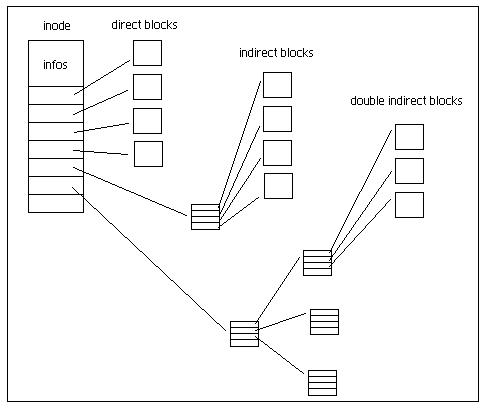
\includegraphics[width=0.65\textwidth]{inode_concept.png}
\caption {The inode concept}
\end{figure}

The file system's inode (on disk) looks as follows:

\vspace{0.3cm}
\begin{tabular}{|l|}
\hline
\textbf{INODE}\\\\\hline
mode (DATA\_FILE or DIRECTORY)\\\hline
size (DATA\_FILE: \#bytes; DIRECTORY: \#entries)\\\hline
timestamp of creation\\\hline
timestamp of last modification\\\hline
pointer to 1st data block\\
...\\
pointer to 30th data block\\\hline
single indirect pointer\\\hline
double indirect pointer\\\hline
\end{tabular}

\begin{code}[kernel/fs/fs\_types.h]
typedef struct d_inode {
		uint16 i_mode;
		uint32 i_size;
		time_t i_create_ts;
		time_t i_modify_ts;
		block_nr i_direct_pointer[NUM_DIRECT_POINTER];
		block_nr i_single_indirect_pointer;
		block_nr i_double_indirect_pointer;
};
\end{code}

\subsubsection{Inode table}
\hypertarget{inodetable}{}
When a file is opened, its inode is located and brought into the inode table \footnote{kernel/fs/inode\_table.h} in memory, where it remains until the file is closed. The inodes in memory have two additional fields, "number" (the inode's ID) and "block address" (the inode's location on disk), being necessary to handle the inode in the inode table or to effectively write it back to disk.

\begin{code}[kernel/fs/fs\_types.h]
typedef struct m_inode {
		inode_nr i_num;
		block_nr i_adr;
		uint16 i_mode;
		uint32 i_size;
		time_t i_create_ts;
		time_t i_modify_ts;
		block_nr i_direct_pointer[NUM_DIRECT_POINTER];
		block_nr i_single_indirect_pointer;
		block_nr i_double_indirect_pointer;
};
\end{code}

\subsubsection{Block caches}
\hypertarget{blockcaches}{}
\textit{POTATOES}' file system uses some single block caches \footnote{kernel/fs/buf.h} to make the handling of read/write processes easier. Mostly, they are used as temporary storages providing the last handled block with a specific format (e.g. address list, memory inode/disk inode, plain data, ...) and offering some meta information.

\begin{code}[kernel/fs/fs\_types.h]
typedef struct block_buffer {
		block_nr block_nr;
		uint8 cache[BLOCK_SIZE];
};
\end{code}

Finally, there are 5 different types of block caches:
\begin{enumerate}
	\item{read\_cache}
	\item{write\_cache}
	\item{addr\_cache (containing 32 bit block addresses)}
	\item{d\_inode\_cache (containing a disk inode)}
	\item{m\_inode\_cache (containing a memory inode)}
\end{enumerate}

\subsubsection{Files}
\hypertarget{filetable}{}
After a requested inode was successfully fetched from disk, a new "file" is created corresponding to the inode and brought into the file table\footnote{kernel/fs/file\_table.h}. The file then builds a bridge between the file handles offered to processes (= process files) and the inodes stored in memory. A file's structure looks like that:

\vspace{0.3cm}
\begin{tabular}{|l|}
\hline
\textbf{FILE}\\\\\hline
global file descriptor\\\hline
pointer to corresponding inode\\\hline
file name (absolute path)\\\hline
file mode (see \hyperlink{inodetable}{"i\_node"})\\\hline
number of opened links\\\hline
\end{tabular}

\begin{code}[kernel/fs/fs\_types.h]
typedef struct file {
		file_nr f_desc;
		m_inode *f_inode;
		char *f_name;
		uint8 f_mode;
		uint16 f_count;
};
\end{code}

\hypertarget{processfiletable}{}
The purpose of a "process file" is to store meta information, e.g. current position within a file, as well as to be an interface between the operating system and the file system. Each process has to create and hold an own process file table managed by the file system. Once there are all process files closed, the file and the inode will be dropped in order to clear up and save memory.

\vspace{0.3cm}
\begin{tabular}{|l|}
\hline
\textbf{PROCESS FILE}\\\\\hline
process file descriptor\\\hline
pointer to global file descriptor\\\hline
file position\\\hline
\end{tabular}

\begin{code}[kernel/fs/fs\_types.h]
typedef struct proc_file {
		file_nr pf_desc;
		file_nr pf_f_desc;
		uint32 pf_pos;
};       
\end{code}
\subsubsection{Directories}
Last but not least, the following figure depicts a single directory entry. Although being a "simple" file, a directory differs in formating its data/entries as follows:

\vspace{0.3cm}
\begin{tabular}{|l|}
\hline
\textbf{DIR ENTRY}\\\\\hline
block number of file's inode\\\hline
file name\\\hline
\end{tabular}

\begin{code}[kernel/fs/fs\_types.h]
typedef struct dir_entry {
		block_nr inode;
		char name[NAME_SIZE];
}
\end{code}
\pagebreak
\section{Applications}

For now every process in \textit{POTATOES} has an own virtual monitor. The focused process is the process with the presently active virtual monitor. You can switch the focus by using the shotrcuts \textbf{Ctrl + '+'} and \textbf{Ctrl + '-'}. These shortcuts are only setting the next/previous virtual monitor as the new active monitor.

\subsection{Shell}
The \textit{POTATOES} shell is the main point of interaction between the user and the system. After boot up the kernel launches one shell instance as a separate process. You can start additional instances in separate vmonitors by pressing \textbf{Ctrl + TAB}.

The shell's user interface consists of a prompt that displays the \textit{current working directory} (which can be changed using the \textbf{cd} command). Commands can take (among other things) \textit{relative} as well as \textit{absolute} paths:

\begin{code}[]
cat /dev/clock
\end{code}

is the same as:

\begin{code}[]
cd /dev
cat clock
\end{code}

To get a list of available commands enter \textbf{cmdlist} and hit return. Another nice feature is \textit{tab-completion} of commands. Simply type the first few letters of a longer command and hit the \textbf{TAB} key to have the shell fill in the rest of the command.

Behind the curtain the shell uses a simple parser to split command strings into arguments (\textbf{void shell\_handle\_command(char *cmd)} in shell\_main.c). Commands are implemented in the source file shell\_cmds.c. Take note that any new commands you implement become available only if you add their function pointer to \textbf{struct shell\_cmd\_t shell\_cmds[]}.

\subsection{Editor}

The embedded \textit{POTATOES} editor is called \textbf{speed}. That is an acronym for \textbf{S}imple \textbf{P}OTATOES/\textbf{E}tiOS \textbf{ED}itor (etiOS is the former project name of \textit{POTATOES}). The editor is not only called simple - it is simple! Speed starts (as every process) an own virtual monitor. The string you see on the editor's monitor while execution will be saved in the opened file on \textbf{ESCAPE}. For now speed only supports the control input of \textbf{ENTER}, \textbf{TAB} and \textbf{BACKSPACE}. In future other features as movement through the data-string using arrow-keys will be added.

\subsection{Snapshot}
Snapshot is a small tool for taking and viewing screenshots in \textit{POTATOES}. The 	functioning of this tool is pretty easy - it just copies the current content of the video memory into a data file. The capture is initialized on the shortcut \textbf{Ctrl + s}. You will be instantly prompted to enter a filename for the new screenshot. To view a screenshot file there is a shell command called \textbf{view}. This command takes control on the active virtual monitor showing only the content of the screenshot file until \textbf{ESCAPE} is pressed.

\subsection{Games}

No operating system is complete without any game to play. Also, interactive games require a lot more resources in comparison to most applications, which makes them an ideal stability and performance test. They are nice to play, as well.

\subsubsection{Pong}

\begin{wrapfigure}{l}{5cm}
\centering
{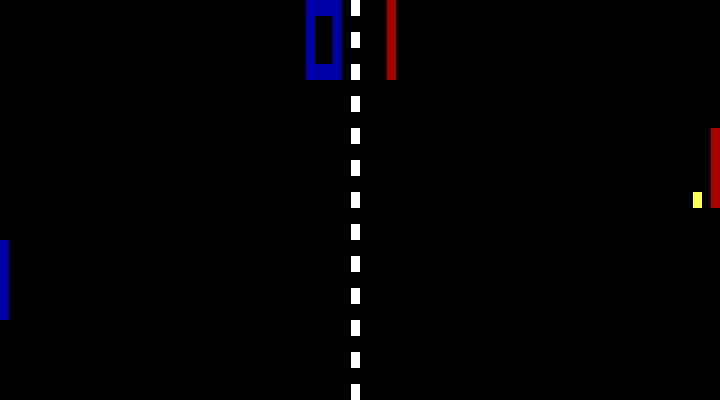
\includegraphics[width=5cm]{pong.png}}
\caption {Pong game}
\end{wrapfigure}

Pong is a simplistic game from the old age of computing, popularized by the American game console manufacturer Atari. 

\textit{POTATOES} contains an implementation of Pong that is also multiplayer capable. You can launch the game by running the \textbf{pong} or \textbf{pong -2p} command in the shell.
Pong's need for fast access to user input as well as high video refresh rate led to the addition of the \textit{keyboard} and \textit{framebuffer} device to \textit{POTATOES}. Also, it is cool and popular with little girls, i.e. my cousin.

\subsubsection{Snake}

\begin{wrapfigure}{r}{5cm}
\centering
{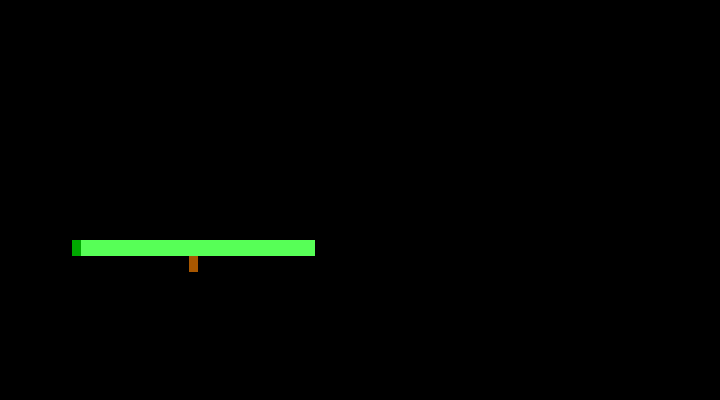
\includegraphics[width=5cm]{snake.png}}
\caption {Snake game}
\end{wrapfigure}

An other game implemented in \textit{POTATOES} is the classic Snake game. You can launch this game by running \textbf{snake} for single- and \textbf{snake -2p} for multiplayer mode.

Snake uses almost the same resources as Pong, in particular the keyboard and the framebuffer device. The most interesting characteristic in the implementation is the reuse of the FIFO-queue developed for the virtual monitors and the devices subsystem. The idea is to represent the snake itself as a FIFO-queue. That makes it really easy to move it on the screen just taking the endmost pixel from the queue and adding a new pixel as the new head of the snake.

\subsection{Brainfuck interpreter}

As an special delicacy \textit{POTATOES} has an own \textbf{brainfuck interpreter}. Brainfuck is an esoteric turing-complete programming language, consisting of only eight commands\footnote{\url{http://en.wikipedia.org/wiki/Brainfuck}}. The corresponding shell command is \textbf{bf [filename]}. It executes the given file which should contain a brainfuck program. 

That is the functionality every interpreter will provide. The brainfuck interpreter in \textit{POTATOES} can do even more. It can interpret single brainfuck commands on the fly. That made it possible to create an interactive brainfuck mode for our shell. It can be launched with the command \textbf{bf -i [sequence]} where [sequence] is an arbitrary sequence of brainfuck command e.g. the simple sequence \textbf{,.[,.]} is a short echo program in brainfuck.  Because of the interactivity we can split this example sequence into single commands:
\begin{code}[]
bf -i ,
bf -i .
bf -i [
bf -i ,
bf -i .
bf -i ]
\end{code}

Executing these commands one after another results in the same echo program as interpreting the whole sequence at once.

\pagebreak
%\lstlistoflistings
\end{document}
